\documentclass{article}
\usepackage{tikz}
\usetikzlibrary{automata, positioning}
\begin{document}
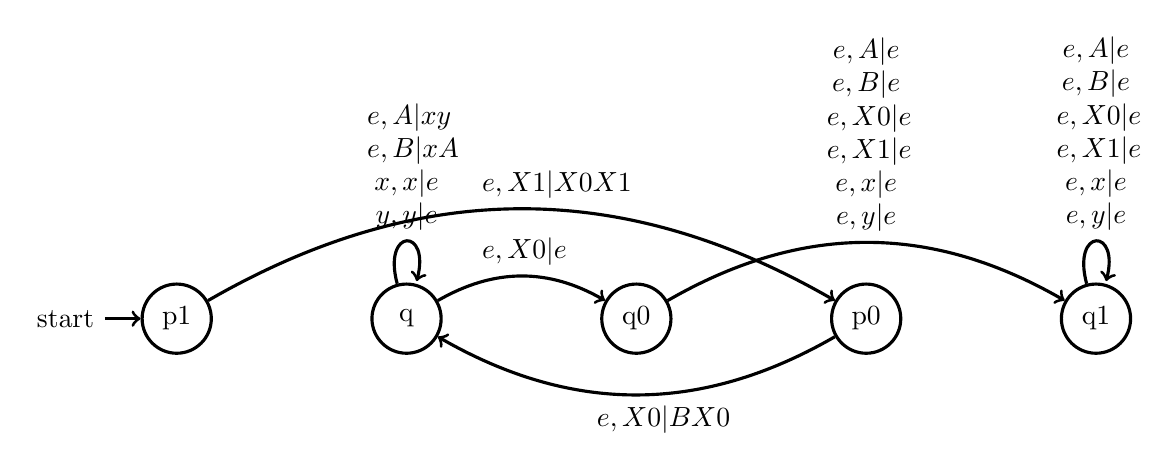
\begin{tikzpicture} [->,auto,node distance=2cm, line width=0.4mm]
\node[state, initial] (p1) {p1};
\node[state] (q) [right =of p1] {q};
\node[state] (q0) [right =of q] {q0};
\node[state] (p0) [right =of q0] {p0};
\node[state] (q1) [right =of p0] {q1};
\path
(q) edge [loop above] node[text width=1cm, align=center] {$e, A | xy$ \\ $e, B | xA$ \\ $x, x | e$ \\ $y, y | e$ \\ } (q)
(q) edge [bend left] node[text width=1cm, align=center] {$e, X0 | e$ \\ } (q0)
(q0) edge [bend left] node[text width=1cm, align=center] {$e, A | e$ \\ $e, B | e$ \\ $e, X0 | e$ \\ $e, X1 | e$ \\ $e, x | e$ \\ $e, y | e$ \\ } (q1)
(p0) edge [bend left] node[text width=1cm, align=center] {$e, X0 | BX0$ \\ } (q)
(q1) edge [loop above] node[text width=1cm, align=center] {$e, A | e$ \\ $e, B | e$ \\ $e, X0 | e$ \\ $e, X1 | e$ \\ $e, x | e$ \\ $e, y | e$ \\ } (q1)
(p1) edge [bend left] node[text width=1cm, align=center] {$e, X1 | X0X1$ \\ } (p0)
;
\end{tikzpicture}
\end{document}
